\documentclass[11pt,a4paper]{ctexart}
\usepackage[a4paper,margin=1in]{geometry}
\usepackage{amsmath,amssymb}
\usepackage{graphicx}
\usepackage{float}
\usepackage{hyperref}
\usepackage{booktabs}

\hypersetup{
  colorlinks=true,
  linkcolor=blue,
  urlcolor=blue
}

\title{$u_0$ 锚定同伦算例图集}
\author{}
\date{\today}

\begin{document}
\maketitle
\tableofcontents

\section*{说明}
这份图集汇总了当前 $u_0$ 锚定同伦 demo 的主要算例。每个算例都给出方程、误差关于 $t$ 的曲线、配对 $(N,p)$ 下误差关于 $N$ 的图，以及一张仿照论文 Table 5.2 的离散结果表。

原问题统一写为
\[
\det(D^2 u(x,y)) = f(x,y), \qquad (x,y)\in \Omega=(0,1)^2,
\]
\[
u(x,y)=g(x,y), \qquad (x,y)\in \partial\Omega.
\]

配对 sweep 统一采用
\[
N = 2,4,6,8,\ldots,32, \qquad
p = 3,5,7,9,\ldots,33, \qquad
t = 10^{-p}.
\]

表中的连续 $L^2$ 与连续 $H^1$ 误差使用高阶 Gauss--Legendre 求积近似。

\clearpage
\section{算例 1：论文算例 5.1（\texttt{paper\_example\_5\_1}）}
\[
\begin{aligned}
u(x,y) &= \exp\!\left(\frac{x^2+y^2}{2}\right),\\
f(x,y) &= \bigl(1+x^2+y^2\bigr)\exp(x^2+y^2),\\
g(x,y) &= \exp\!\left(\frac{x^2+y^2}{2}\right), \qquad (x,y)\in\partial\Omega.
\end{aligned}
\]
\begin{figure}[H]
  \centering
  
\includegraphics[width=0.88\textwidth]{../u0_anchor_monge_ampere_homotopy_paper_example_5_1_gallery_cn_tables/u0_anchor_homotopy_error_curves.png}
  \caption{算例 \texttt{paper\_example\_5\_1} 的误差关于 $t$ 的曲线。}
\end{figure}
\begin{figure}[H]
  \centering
  
\includegraphics[width=0.88\textwidth]{../u0_anchor_monge_ampere_homotopy_paper_example_5_1_N_sweep_gallery_cn_contnorm_tables_paired_p_to_32/u0_anchor_error_vs_N.png}
  \caption{算例 \texttt{paper\_example\_5\_1} 在配对 $(N,p)$ 下的误差关于 $N$ 的图。}
\end{figure}
\begin{table}[H]
  \centering
  \small
  \caption{算例 \texttt{paper\_example\_5\_1} 的离散结果表。}
  \begin{tabular}{r r r r}
    \toprule
    $N$ & 连续 $L^2$ 误差 & 连续 $H^1$ 误差 & cpu(s) \\
    \midrule
2 & 4.736E-3 & 2.279E-2 & 10.2138 \\
4 & 7.254E-5 & 6.194E-4 & 5.8635 \\
6 & 7.479E-7 & 9.358E-6 & 5.5097 \\
8 & 5.956E-9 & 9.831E-8 & 5.4376 \\
10 & 3.855E-11 & 7.905E-10 & 5.3628 \\
12 & 2.64E-13 & 6.156E-12 & 5.3466 \\
14 & 1.72E-14 & 3.533E-13 & 5.4909 \\
16 & 1.493E-14 & 9.951E-13 & 5.7584 \\
18 & 3.055E-14 & 3.289E-12 & 5.9342 \\
20 & 1.217E-13 & 3.768E-12 & 6.3693 \\
22 & 1.08E-13 & 3.558E-12 & 6.9907 \\
24 & 4.609E-14 & 2.809E-12 & 7.6391 \\
26 & 1.774E-13 & 6.056E-12 & 8.4050 \\
28 & 2.964E-13 & 1.224E-11 & 9.7995 \\
30 & 1.626E-13 & 9.774E-12 & 11.6566 \\
32 & 8.402E-14 & 4.941E-12 & 14.0969 \\
    \\bottomrule
  \end{tabular}
\end{table}

\clearpage
\section{算例 2：温和分离指数算例（\texttt{mild\_exp\_separable}）}
\[
\begin{aligned}
u(x,y) &= e^{0.2x}+e^{0.2y}-2,\\
f(x,y) &= 0.0016\,e^{0.2(x+y)},\\
g(x,y) &= e^{0.2x}+e^{0.2y}-2, \qquad (x,y)\in\partial\Omega.
\end{aligned}
\]
\begin{figure}[H]
  \centering
  
\includegraphics[width=0.88\textwidth]{../u0_anchor_monge_ampere_homotopy_mild_exp_separable_gallery_cn_tables/u0_anchor_homotopy_error_curves.png}
  \caption{算例 \texttt{mild\_exp\_separable} 的误差关于 $t$ 的曲线。}
\end{figure}
\begin{figure}[H]
  \centering
  
\includegraphics[width=0.88\textwidth]{../u0_anchor_monge_ampere_homotopy_mild_exp_separable_N_sweep_gallery_cn_contnorm_tables_paired_p_to_32/u0_anchor_error_vs_N.png}
  \caption{算例 \texttt{mild\_exp\_separable} 在配对 $(N,p)$ 下的误差关于 $N$ 的图。}
\end{figure}
\begin{table}[H]
  \centering
  \small
  \caption{算例 \texttt{mild\_exp\_separable} 的离散结果表。}
  \begin{tabular}{r r r r}
    \toprule
    $N$ & 连续 $L^2$ 误差 & 连续 $H^1$ 误差 & cpu(s) \\
    \midrule
2 & 1.055E-6 & 4.719E-6 & 5.6232 \\
4 & 1.305E-10 & 9.638E-10 & 5.2751 \\
6 & 2.042E-13 & 9.304E-13 & 5.3349 \\
8 & 3.629E-15 & 4.367E-14 & 5.3229 \\
10 & 2.36E-15 & 5.193E-14 & 5.3743 \\
12 & 1.153E-14 & 2.127E-13 & 5.3645 \\
14 & 2.665E-15 & 4.936E-14 & 5.3866 \\
16 & 2.779E-15 & 1.769E-13 & 5.6754 \\
18 & 5.303E-15 & 5.621E-13 & 5.8234 \\
20 & 2.202E-14 & 6.31E-13 & 6.0331 \\
22 & 1.038E-14 & 4.127E-13 & 6.5569 \\
24 & 7.149E-15 & 4.382E-13 & 6.9780 \\
26 & 3.143E-14 & 1.013E-12 & 7.9933 \\
28 & 5.172E-14 & 2.052E-12 & 8.8547 \\
30 & 2.905E-14 & 1.584E-12 & 10.3047 \\
32 & 1.562E-14 & 6.748E-13 & 12.5836 \\
    \\bottomrule
  \end{tabular}
\end{table}

\clearpage
\section{算例 3：混合多项式凸算例（\texttt{mixed\_polynomial\_convex}）}
\[
\begin{aligned}
u(x,y) &= \frac12(x^2+y^2)+0.01(x^6+y^6)+0.01x^2y^2,\\
f(x,y) &= \bigl(1+0.3x^4+0.02y^2\bigr)\bigl(1+0.3y^4+0.02x^2\bigr)-(0.04xy)^2,\\
g(x,y) &= \frac12(x^2+y^2)+0.01(x^6+y^6)+0.01x^2y^2, \qquad (x,y)\in\partial\Omega.
\end{aligned}
\]
\begin{figure}[H]
  \centering
  
\includegraphics[width=0.88\textwidth]{../u0_anchor_monge_ampere_homotopy_mixed_polynomial_convex_gallery_cn_tables/u0_anchor_homotopy_error_curves.png}
  \caption{算例 \texttt{mixed\_polynomial\_convex} 的误差关于 $t$ 的曲线。}
\end{figure}
\begin{figure}[H]
  \centering
  
\includegraphics[width=0.88\textwidth]{../u0_anchor_monge_ampere_homotopy_mixed_polynomial_convex_N_sweep_gallery_cn_contnorm_tables_paired_p_to_32/u0_anchor_error_vs_N.png}
  \caption{算例 \texttt{mixed\_polynomial\_convex} 在配对 $(N,p)$ 下的误差关于 $N$ 的图。}
\end{figure}
\begin{table}[H]
  \centering
  \small
  \caption{算例 \texttt{mixed\_polynomial\_convex} 的离散结果表。}
  \begin{tabular}{r r r r}
    \toprule
    $N$ & 连续 $L^2$ 误差 & 连续 $H^1$ 误差 & cpu(s) \\
    \midrule
2 & 6.025E-4 & 2.743E-3 & 5.2341 \\
4 & 1.164E-5 & 9.326E-5 & 5.2505 \\
6 & 2.522E-13 & 1.152E-12 & 5.3038 \\
8 & 6.274E-15 & 7.856E-14 & 5.3702 \\
10 & 2.768E-15 & 1.049E-13 & 5.3394 \\
12 & 2.136E-14 & 4.519E-13 & 5.3996 \\
14 & 4.373E-15 & 8.348E-14 & 5.5011 \\
16 & 5.356E-15 & 3.536E-13 & 5.7083 \\
18 & 1.027E-14 & 1.122E-12 & 5.8787 \\
20 & 4.206E-14 & 1.273E-12 & 6.2446 \\
22 & 1.894E-14 & 7.49E-13 & 6.8070 \\
24 & 1.618E-14 & 8.88E-13 & 7.4938 \\
26 & 6.184E-14 & 2.122E-12 & 10.6130 \\
28 & 1.032E-13 & 4.275E-12 & 16.6748 \\
30 & 5.737E-14 & 3.237E-12 & 20.4539 \\
32 & 3.1E-14 & 1.411E-12 & 25.7441 \\
    \\bottomrule
  \end{tabular}
\end{table}

\clearpage
\section{算例 4：温和六次凸算例（\texttt{mild\_sextic\_convex}）}
\[
\begin{aligned}
u(x,y) &= \frac12(x^2+y^2)+0.02(x^6+y^6),\\
f(x,y) &= \bigl(1+0.6x^4\bigr)\bigl(1+0.6y^4\bigr),\\
g(x,y) &= \frac12(x^2+y^2)+0.02(x^6+y^6), \qquad (x,y)\in\partial\Omega.
\end{aligned}
\]
\begin{figure}[H]
  \centering
  
\includegraphics[width=0.88\textwidth]{../u0_anchor_monge_ampere_homotopy_mild_sextic_convex_gallery_cn_tables/u0_anchor_homotopy_error_curves.png}
  \caption{算例 \texttt{mild\_sextic\_convex} 的误差关于 $t$ 的曲线。}
\end{figure}
\begin{figure}[H]
  \centering
  
\includegraphics[width=0.88\textwidth]{../u0_anchor_monge_ampere_homotopy_mild_sextic_convex_N_sweep_gallery_cn_contnorm_tables_paired_p_to_32/u0_anchor_error_vs_N.png}
  \caption{算例 \texttt{mild\_sextic\_convex} 在配对 $(N,p)$ 下的误差关于 $N$ 的图。}
\end{figure}
\begin{table}[H]
  \centering
  \small
  \caption{算例 \texttt{mild\_sextic\_convex} 的离散结果表。}
  \begin{tabular}{r r r r}
    \toprule
    $N$ & 连续 $L^2$ 误差 & 连续 $H^1$ 误差 & cpu(s) \\
    \midrule
2 & 1.197E-3 & 5.45E-3 & 7.7193 \\
4 & 2.322E-5 & 1.863E-4 & 7.7848 \\
6 & 9.583E-13 & 4.356E-12 & 7.0934 \\
8 & 1.299E-14 & 9.582E-14 & 5.5050 \\
10 & 2.82E-15 & 1.057E-13 & 5.5192 \\
12 & 2.162E-14 & 4.595E-13 & 5.5465 \\
14 & 4.276E-15 & 8.483E-14 & 5.6445 \\
16 & 5.282E-15 & 3.562E-13 & 5.7474 \\
18 & 1.041E-14 & 1.136E-12 & 5.9888 \\
20 & 4.258E-14 & 1.289E-12 & 6.2728 \\
22 & 1.927E-14 & 7.598E-13 & 6.7920 \\
24 & 1.685E-14 & 8.985E-13 & 7.2987 \\
26 & 6.263E-14 & 2.141E-12 & 8.0838 \\
28 & 1.045E-13 & 4.327E-12 & 9.3361 \\
30 & 5.759E-14 & 3.279E-12 & 11.1162 \\
32 & 3.091E-14 & 1.425E-12 & 13.2005 \\
    \\bottomrule
  \end{tabular}
\end{table}

\clearpage
\section{算例 5：高斯鼓包凸算例（\texttt{gaussian\_bump\_convex}）}
\[
\begin{aligned}
u(x,y) &= \frac12(x^2+y^2)+0.03\,e^{-6((x-\tfrac12)^2+(y-\tfrac12)^2)},\\
f(x,y) &= u_{xx}u_{yy}-u_{xy}^2,\\
g(x,y) &= \frac12(x^2+y^2)+0.03\,e^{-6((x-\tfrac12)^2+(y-\tfrac12)^2)}, \qquad (x,y)\in\partial\Omega.
\end{aligned}
\]
\begin{figure}[H]
  \centering
  
\includegraphics[width=0.88\textwidth]{../u0_anchor_monge_ampere_homotopy_gaussian_bump_convex_gallery_cn_tables/u0_anchor_homotopy_error_curves.png}
  \caption{算例 \texttt{gaussian\_bump\_convex} 的误差关于 $t$ 的曲线。}
\end{figure}
\begin{figure}[H]
  \centering
  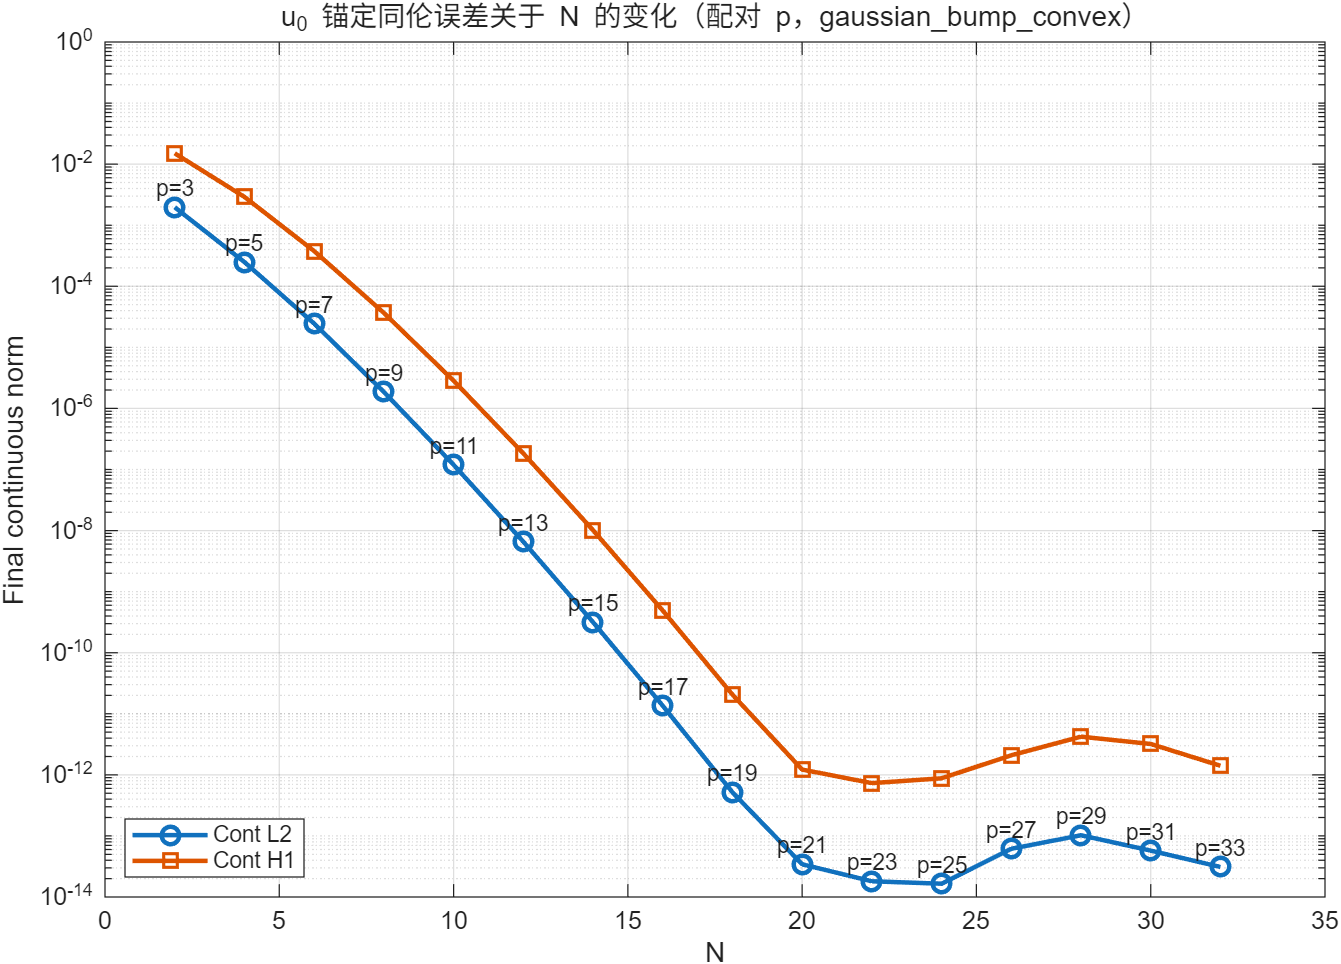
\includegraphics[width=0.88\textwidth]{../u0_anchor_monge_ampere_homotopy_gaussian_bump_convex_N_sweep_gallery_cn_contnorm_tables_paired_p_to_32/u0_anchor_error_vs_N.png}
  \caption{算例 \texttt{gaussian\_bump\_convex} 在配对 $(N,p)$ 下的误差关于 $N$ 的图。}
\end{figure}
\begin{table}[H]
  \centering
  \small
  \caption{算例 \texttt{gaussian\_bump\_convex} 的离散结果表。}
  \begin{tabular}{r r r r}
    \toprule
    $N$ & 连续 $L^2$ 误差 & 连续 $H^1$ 误差 & cpu(s) \\
    \midrule
2 & 1.967E-3 & 1.505E-2 & 5.3595 \\
4 & 2.492E-4 & 2.91E-3 & 5.4123 \\
6 & 2.452E-5 & 3.771E-4 & 5.4251 \\
8 & 1.86E-6 & 3.665E-5 & 5.4727 \\
10 & 1.196E-7 & 2.846E-6 & 5.4466 \\
12 & 6.579E-9 & 1.838E-7 & 5.5864 \\
14 & 3.168E-10 & 1.016E-8 & 5.6359 \\
16 & 1.355E-11 & 4.902E-10 & 5.8132 \\
18 & 5.178E-13 & 2.062E-11 & 5.9374 \\
20 & 3.433E-14 & 1.221E-12 & 6.3161 \\
22 & 1.808E-14 & 7.319E-13 & 6.7902 \\
24 & 1.651E-14 & 8.781E-13 & 7.7274 \\
26 & 6.162E-14 & 2.092E-12 & 8.3379 \\
28 & 1.026E-13 & 4.22E-12 & 9.5014 \\
30 & 5.749E-14 & 3.205E-12 & 11.2333 \\
32 & 3.102E-14 & 1.41E-12 & 13.5330 \\
    \\bottomrule
  \end{tabular}
\end{table}

\clearpage
\section{算例 6：四次凸算例（\texttt{quartic\_convex}）}
\[
\begin{aligned}
u(x,y) &= \frac12(x^2+y^2)+x^4+y^4,\\
f(x,y) &= \bigl(1+12x^2\bigr)\bigl(1+12y^2\bigr),\\
g(x,y) &= \frac12(x^2+y^2)+x^4+y^4, \qquad (x,y)\in\partial\Omega.
\end{aligned}
\]

当前版本对该算例采用了专门的分离型 anchor，以改善高 $N$ 下的稳定性。

\begin{figure}[H]
  \centering
  
\includegraphics[width=0.88\textwidth]{../u0_anchor_monge_ampere_homotopy_quartic_convex_gallery_cn_tables/u0_anchor_homotopy_error_curves.png}
  \caption{算例 \texttt{quartic\_convex} 的误差关于 $t$ 的曲线。}
\end{figure}
\begin{figure}[H]
  \centering
  
\includegraphics[width=0.88\textwidth]{../u0_anchor_monge_ampere_homotopy_quartic_convex_N_sweep_gallery_cn_contnorm_tables_paired_p_to_32/u0_anchor_error_vs_N.png}
  \caption{算例 \texttt{quartic\_convex} 在配对 $(N,p)$ 下的误差关于 $N$ 的图。}
\end{figure}
\begin{table}[H]
  \centering
  \small
  \caption{算例 \texttt{quartic\_convex} 的离散结果表。}
  \begin{tabular}{r r r r}
    \toprule
    $N$ & 连续 $L^2$ 误差 & 连续 $H^1$ 误差 & cpu(s) \\
    \midrule
2 & 1.403E-2 & 6.309E-2 & 5.4036 \\
4 & 6.41E-15 & 7.567E-14 & 5.4305 \\
6 & 1.383E-14 & 1.747E-13 & 5.4500 \\
8 & 1.145E-14 & 1.91E-13 & 5.4510 \\
10 & 7.232E-15 & 2.794E-13 & 5.4590 \\
12 & 5.286E-14 & 1.213E-12 & 5.4535 \\
14 & 9.732E-15 & 2.043E-13 & 5.5584 \\
16 & 1.364E-14 & 9.364E-13 & 5.5648 \\
18 & 2.599E-14 & 2.89E-12 & 5.7464 \\
20 & 1.055E-13 & 3.434E-12 & 5.9090 \\
22 & 5.419E-14 & 1.97E-12 & 6.2289 \\
24 & 4.158E-14 & 2.316E-12 & 6.5087 \\
26 & 1.556E-13 & 5.719E-12 & 7.0468 \\
28 & 2.608E-13 & 1.158E-11 & 7.7670 \\
30 & 1.42E-13 & 8.683E-12 & 9.2503 \\
32 & 7.648E-14 & 3.781E-12 & 10.0121 \\
    \\bottomrule
  \end{tabular}
\end{table}

\end{document}
